\subsection{Edytor punktów końcowych}

Edytor punktów końcowych to jedna z ważniejszych funkcji programu. Umożliwia
administratorowi definiowanie punktów końcowych HTTP, których wywołanie
spowoduje wykonanie napisanego przez administratora drzewa zapytań SQL.

Dane wynikające z wykonania drzewa zapytań zostaną zwrócone w formacie json.
Struktura zwróconego dokumentu json będzie odpowiadała strukturze drzewa zapytań
SQL zaprojektowanego przez administratora.

Zapytania podrzędne mogą korzystać z danych wynikających z zapytania
nadrzędnego. Dane można pobrać za pomocą specjalnej składni, która zostanie
sparsowana przez program. Dane zostaną umieszczone w zapytaniach nadrzędnych w
sposób zabezpieczony przed atakami SQL injection.

Składnia dostępu do danych była zaprojektowana z myślą o prostocie, powinna być
trywialna w nauce dla kogoś, kto ma nawet podstawową wiedzę o językach
programowania. Składa się z dwóch wariantów:

\begin{enumerate}

    \item Wariant dostępu do danych przychodzących w zapytaniu HTTP wygląda
    następująco:

        \begin{enumerate}
            
            \item rozpoczęcie \verb|${|,

            \item prefiks \verb|req.|,

            \item nazwa zmiennej,

            \item zakończenie \verb|}|.
            
        \end{enumerate}

        Przykładowo, dostęp do pola ``nazwa'' wygląda tak: \verb|${req.nazwa}|.

    \item Wariant dostępu do danych wynikających z zapytań nadrzędnych wygląda
        następująco:

        \begin{enumerate}
            
            \item rozpoczęcie \verb|${|,

            \item jeden, lub więcej prefiksów \verb|super.|,

            \item nazwa zmiennej,

            \item zakończenie \verb|}|.
            
        \end{enumerate}

        Przykładowo, dostęp do pola ``user\_id'' będącego wynikiem zapytania
        nadrzędnego do zapytania nadrzędnego wygląda tak:
        \verb|${super.super.user_id}|.

\end{enumerate}

Jeśli administrator potrzebuje danych do zapytań podrzędnych, ale nie chce, żeby
były umieszczone w odpowiedzi HTTP, powinien nazwać je tak, by ich nazwa
zaczynała się od prefiksu ``\verb|private_|''. Pola o takiej nazwie można
wykorzystywać w zapytaniach podrzędnych (na przykład
\verb|${super.private_user_id}|), ale nie będą zwrócone w odpowiedzi HTTP.

Działanie i odporność na ataki SQL injection parsera SQL wchodzącego w skład
programu można zrozumieć na przykładzie zawartym w teście jednostkowym
zamieszczonym w listingu \ref{parsingTestListing}.

Sparsowane zapytania SQL składają się z SQL zawierającego odniesienia do
parametrów w składni specyficznej dla bazy danych Postgres
\cite{PostgresPrepareStatement} i listy ciągów znaków, które umożliwią
znalezienie zmiennej w czasie wykonywania drzewa zapytań SQL.

\lstinputlisting[
    float=h!,
    frame=tb,
    label={parsingTestListing},
    caption={Test sprawdzający poprawność parsowania SQL zawierającego
    odniesienia do zmiennych}
]{./code/parsingTest.rs}

Interfejs edytora punktów końcowych zawiera menu rozwijane, które pozwala na
wybór edytowania już istniejącego punktu końcowego, lub tworzenia nowego punktu
końcowego.

Poniżej znajduje się formularz, za pomocą którego tworzony jest punkt końcowy.
Pierwszym elementem formularza jest pole tekstowe, do którego należy wpisać
ścieżkę punktu końcowego. Poniżej znajduje się menu, którego należy użyć do
ustawienia akceptowanych metod HTTP. Opcje to GET, POST i ANY. Wybranie opcji
ANY powoduje akceptowanie zapytań o dowolnej metodzie HTTP.

Kolejnym elementem jest menu, gdzie administrator może ustawić listę grup
użytkowników, które będą miały dostęp do edytowanego punktu końcowego.

Kolejnym, najbardziej skomplikowanym, elementem jest edytor drzewa zapytań SQL.
Administrator może tworzyć kilka niezależnych drzew. Umożliwia to opcja ``New
independent query''. Każdy węzeł drzewa powinien mieć nazwę, która zostanie
użyta, jako klucz w mapie węzłów w wynikowym dokumencie json.

Węzły będące liśćmi można usunąć za pomocą przycisku ``delete''. W celu
zapobiegnięcia niezamierzonego skasowania pracy, węzły posiadające podzapytania
nie posiadają opcji usunięcia. W celu usunięcia tych węzłów, należy najpierw
usunąć ich wszystkie węzły podrzędne.

Każdy węzeł posiada opcję dodania nowego węzła podrzędnego. Można to zrobić za
pomocą przycisku ``New child''.\\

Opisany do tej pory interfejs widać na rysunku \ref{endpointCreationFigure}.\\

\begin{figure}[h]
    \centering
    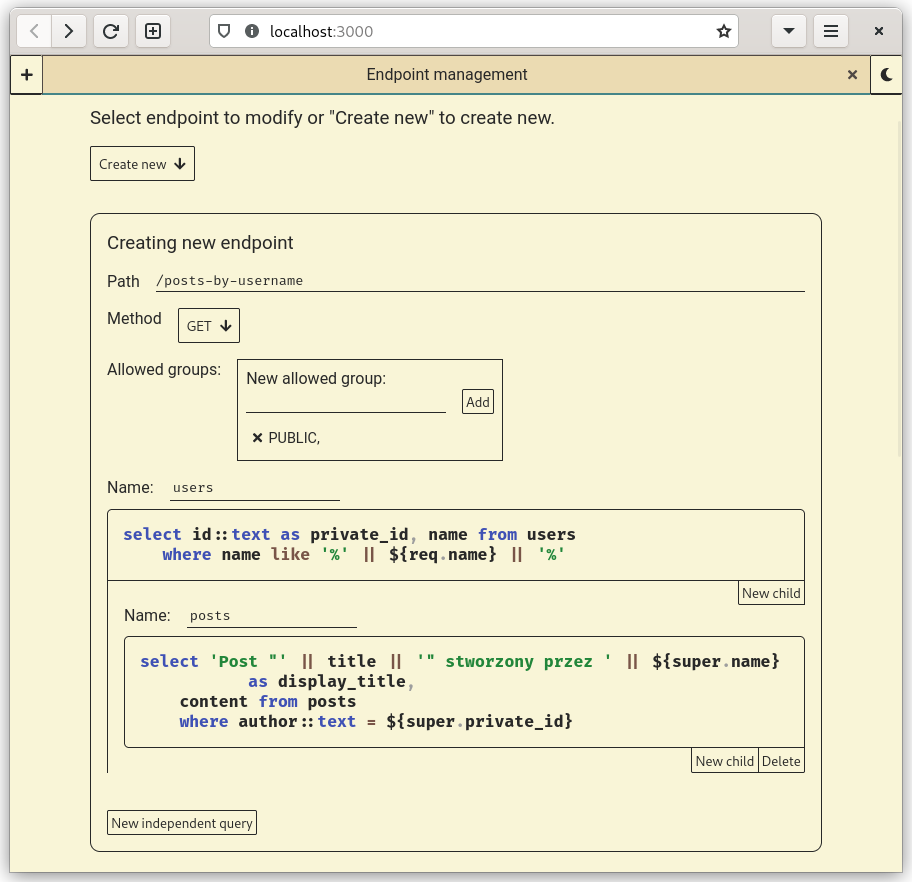
\includegraphics[width=0.8\textwidth]{./img/endpoint_creation.png}
    \caption{Interfejs tworzenia nowego punktu końcowego}
    \label{endpointCreationFigure}
\end{figure}

Program implementuje funkcjonalność mającą na celu umożliwienie administratorowi
wygodnego testowania tworzonych punktów końcowych. Pod edytorem punktu końcowego
znajduje się edytor danych testowych. Umożliwia on tworzenie mapy zmiennych,
które będą traktowane, jak wartości formularza przychodzącego w zapytaniu HTTP.

Testowe wykonanie drzewa zapytań SQL używa transakcji, która jest cofana przed
zwrotem wynikowego dokumentu json. Wynikowy dokument json jest wyświetlany na
dole interfejsu. Wynik testowania punktu końcowego widać na rysunku
\ref{endpointTestingFigure}.

\begin{figure}[h]
    \centering
    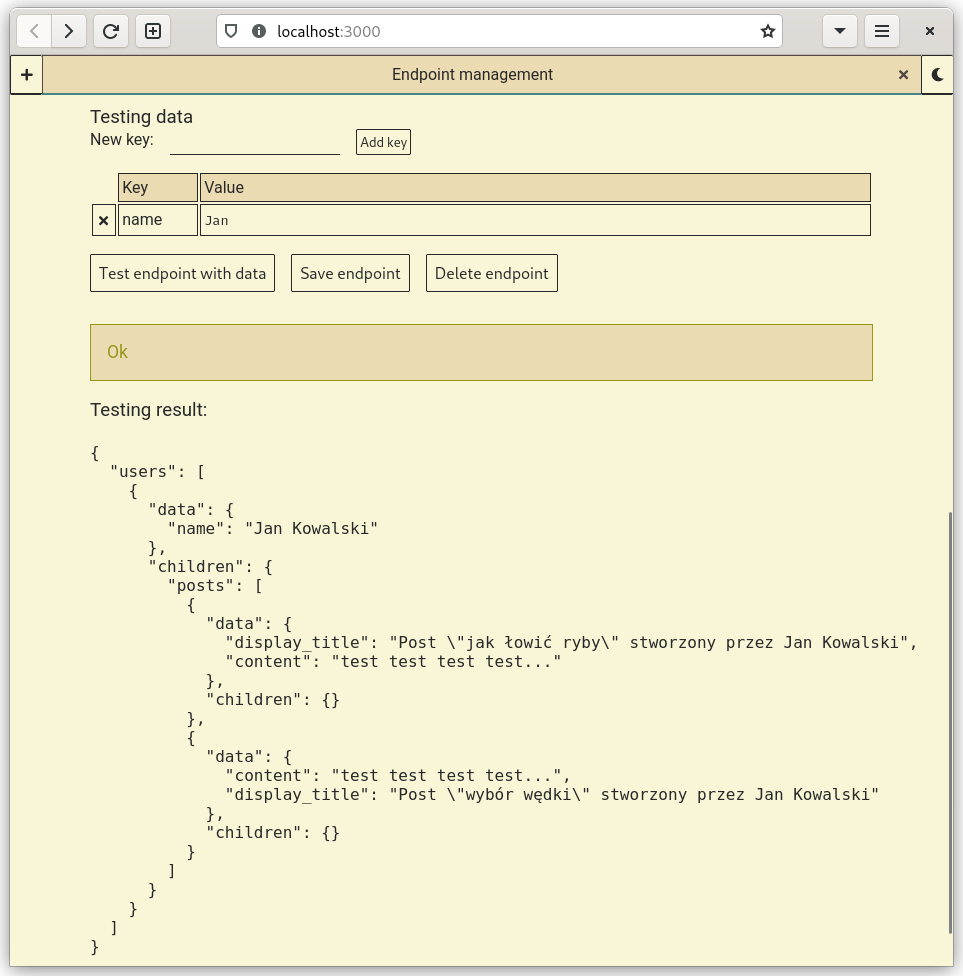
\includegraphics[width=0.8\textwidth]{./img/endpoint_testing.png}
    \caption{Interfejs testowania tworzonego punktu końcowego}
    \label{endpointTestingFigure}
\end{figure}

Zapisane punkty końcowe będą dostępne pod adresem \verb|/endpoint/<ścieżka punktu końcowego>|.
Wywołanie zapisanego punktu końcowego z przeglądarki Firefox - poza panelem
administratora widać na rysunku \ref{endpointFirefoxFigure}.

\begin{figure}[h]
    \centering
    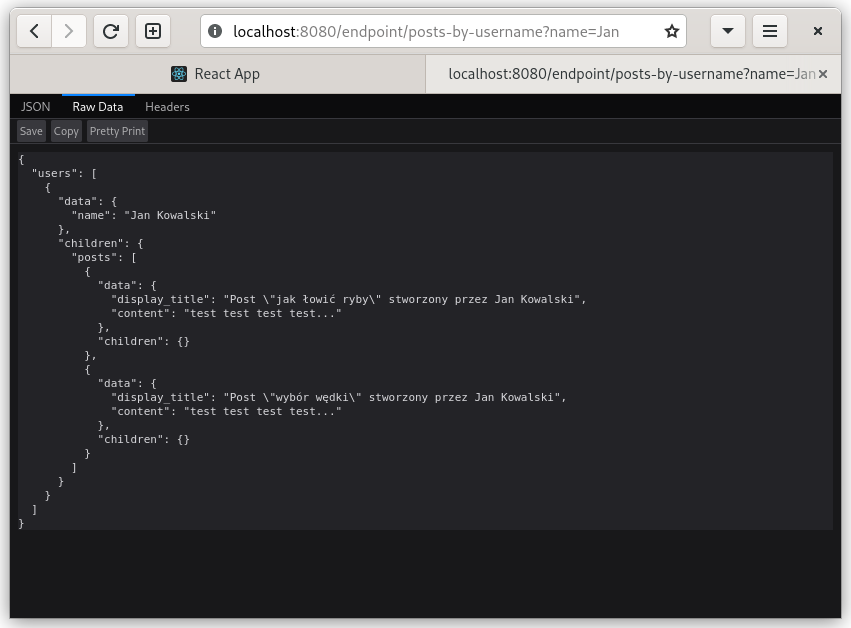
\includegraphics[width=0.7\textwidth]{./img/endpoint_firefox.png}
    \caption{Wywołanie punktu końcowego w przeglądarce Firefox}
    \label{endpointFirefoxFigure}
\end{figure}
